\documentclass{article}
\usepackage[utf8]{inputenc}
\usepackage[russian]{babel}
\usepackage{graphicx}
\usepackage{amsmath}
\usepackage{breqn}
\usepackage{wrapfig}
\usepackage{float}
\usepackage{multirow}
\usepackage{caption}
\usepackage{subcaption}

\graphicspath{ {./data/images} }
\author{Александр Романов Б01-107}
\date{}
\title{3.7.1 Скин-эффект в полом цилиндре}

\begin{document}
\maketitle
\section{Введение}
\subsection{Цель работы}
Исследование проникновения переменного магнитного поля в медный полый цилиндр.
\subsection{В работе используются}
Генератор звуковой частоты, соленоид, намотанный на полый цилиндрический каркас из диэлектрика,
медный экран в виде трубки, измерительная катушка, амперметр, вольтметр, осциллограф. 
\begin{figure}[H]
    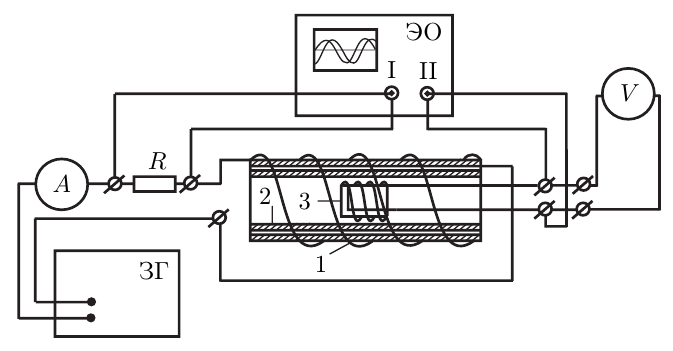
\includegraphics[width=\textwidth]{scheme.png}
    \caption{Схема экспериментальной установки}
\end{figure}

\section{Работа}

\subsection{Подготовка}
Приняв проводимость меди для оценки равной \( \sigma = 5\cdot 10^{7}\; S/m \) расчитаем частоту \( \nu_h\; Hz \),
при которой толщина стенок экрана равна скиновой длине \( \delta = h = 1.5\; mm \). По формуле:
\[ \delta = \sqrt{\frac{2}{\omega \sigma \mu_0}} \Rightarrow \nu_h = \frac{1}{\pi\sigma\mu_0 h^2} = 2250\; Hz \]
\subsection{Измерения в диапазоне \((0.01\nu_h - 0.05\nu_h)\)}
Получим знависимость соотношения \( \xi = U/(\nu I) \) от частоты \(\nu\):
\begin{table}[H]
    \centering
    \begin{tabular}{|c|c|c|c|}
    \hline
    \(\nu\), Hz & U, V  & I, A  & \(\xi = U/(\nu I)\) \\\hline
    22.5 & 0.195 & 0.461 & 0.0188   \\\hline
    31.5 & 0.269 & 0.457 & 0.0187   \\\hline
    40.5 & 0.338 & 0.453 & 0.0184   \\\hline
    49.5 & 0.403 & 0.448 & 0.0182   \\\hline
    58.5 & 0.463 & 0.442 & 0.0179   \\\hline
    67.5 & 0.518 & 0.436 & 0.0176   \\\hline
    76.5 & 0.569 & 0.43  & 0.0173   \\\hline
    85.5 & 0.614 & 0.423 & 0.0170   \\\hline
    94.5 & 0.654 & 0.418 & 0.0166   \\\hline
    103.5& 0.69  & 0.412 & 0.0162   \\\hline
    112.5& 0.723 & 0.406 & 0.0158   \\\hline
    \end{tabular}
\end{table}

\begin{figure}[H]
    \centering
    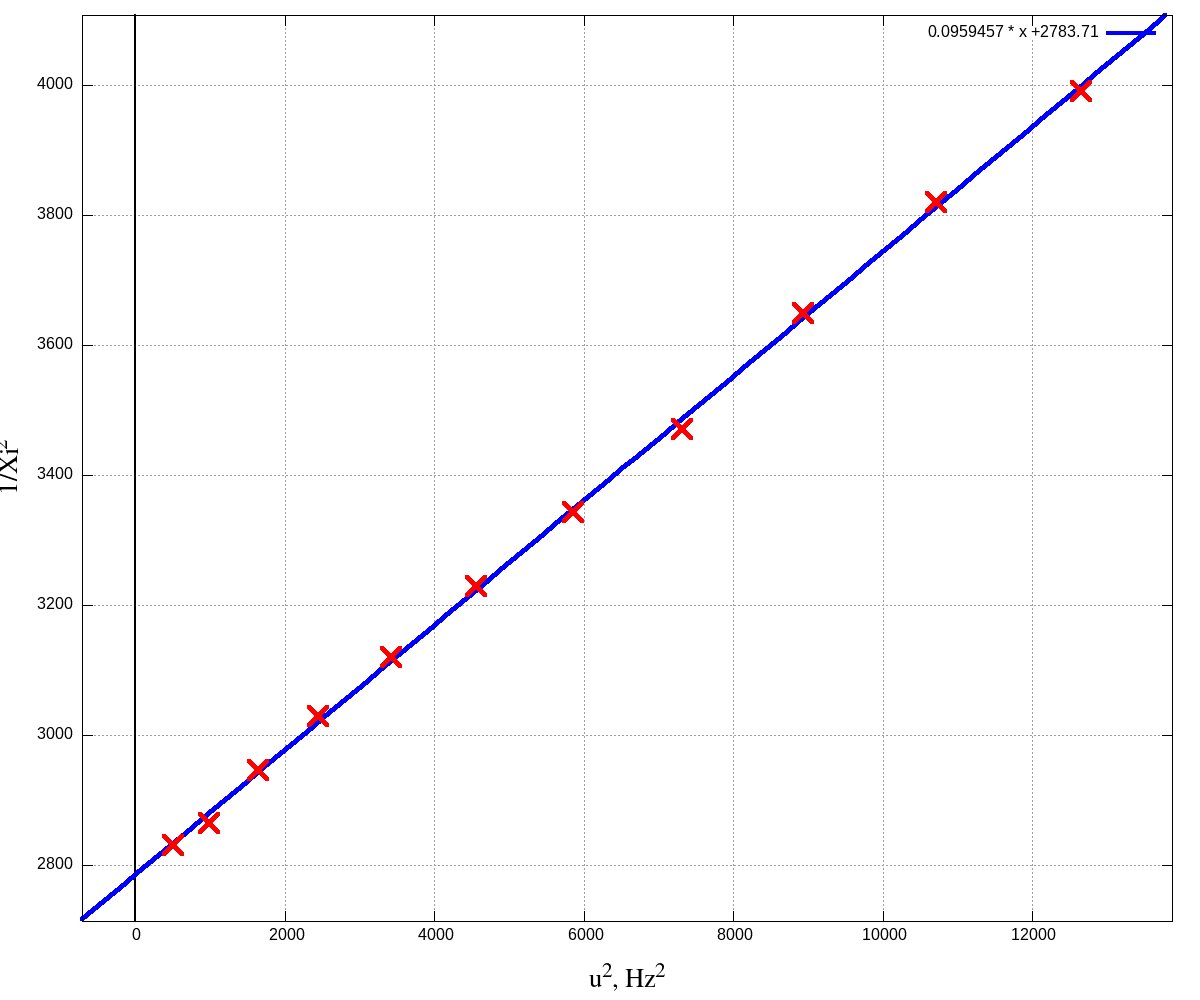
\includegraphics[width=0.8\textwidth]{1.png}
    \caption{график \( \xi(\nu) \)}
\end{figure}

Получена зависимость вида \( \xi = ax + b \):
\[ a = (-3.4\cdot 10^{-5} \pm 1.2\cdot 10^{-6}) \]
\[ b = (0.02 \pm 3.4\cdot 10^{-5}) \]
\subsection{Измерения в диапазоне \((0.05\nu_h - 0.5\nu_h)\)}
Исследуем зависимости \(\xi\) и \(\psi\) от \(\nu\):
\begin{table}[H]
    \centering
    \begin{tabular}{|c|c|c|c|c|}
    \hline
    \(\nu\), Hz & U, V  & I, A  & \(\psi\), rad & \(\xi = U/(\nu I)\) \\\hline
    112.5  & 0.721 & 0.404 & 3.70 & 0.0159\\\hline
    128.5  & 0.769 & 0.394 & 3.87 & 0.0152\\\hline
    144.5  & 0.809 & 0.386 & 4.06 & 0.0145\\\hline
    160.5  & 0.841 & 0.378 & 4.05 & 0.0139\\\hline
    176.5  & 0.868 & 0.371 & 4.04 & 0.0133\\\hline
    192.5  & 0.89  & 0.366 & 4.11 & 0.0126\\\hline
    208.5  & 0.908 & 0.361 & 4.06 & 0.0121\\\hline
    225 & 0.923 & 0.356 & 4.05 & 0.0115\\\hline
    315 & 0.967 & 0.338 & 4.32 & 0.0091\\\hline
    405 & 0.98  & 0.327 & 4.27 & 0.0074\\\hline
    495 & 0.979 & 0.318 & 4.29 & 0.0062\\\hline
    585 & 0.971 & 0.311 & 4.43 & 0.0053\\\hline
    675 & 0.959 & 0.304 & 4.61 & 0.0047\\\hline
    765 & 0.943 & 0.297 & 4.59 & 0.0042\\\hline
    855 & 0.927 & 0.291 & 4.68 & 0.0037\\\hline
    945 & 0.908 & 0.284 & 4.62 & 0.0034\\\hline
    1035& 0.888 & 0.278 & 4.71 & 0.0031\\\hline
    \end{tabular}
\end{table}

\begin{figure}[H]
    \centering
    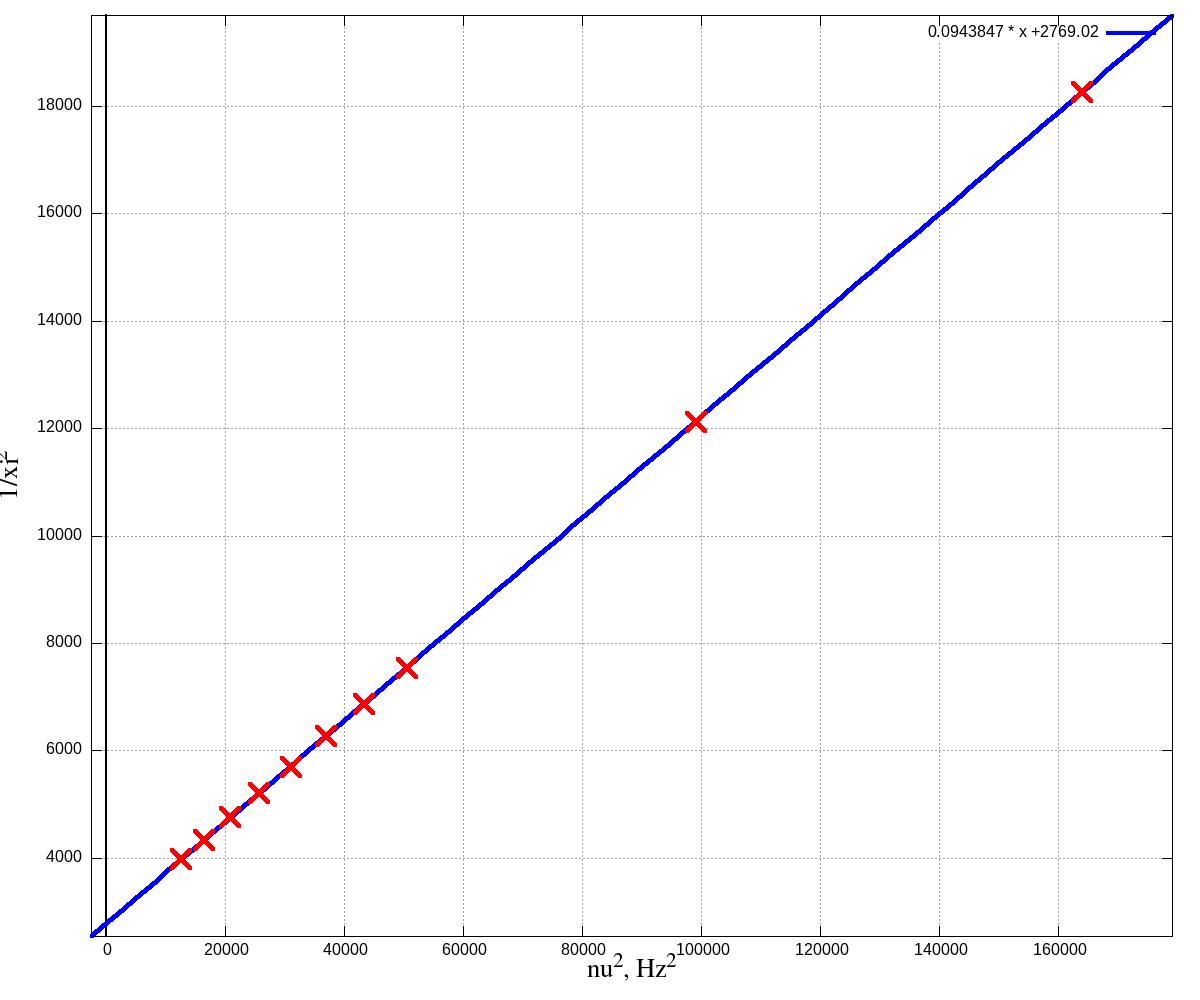
\includegraphics[width=0.8\textwidth]{2.png}
    \caption{график \( \xi(\nu) \)}
\end{figure}

Опроксимируем многочленом 3 степени:
\[ \xi = 0.02 - 5.6\cdot 10^{-6}\nu + 6.4\cdot 10^{-8}\nu^2 - 2.6\cdot 10^{-11}\nu^3 \]

\begin{figure}[H]
    \centering
    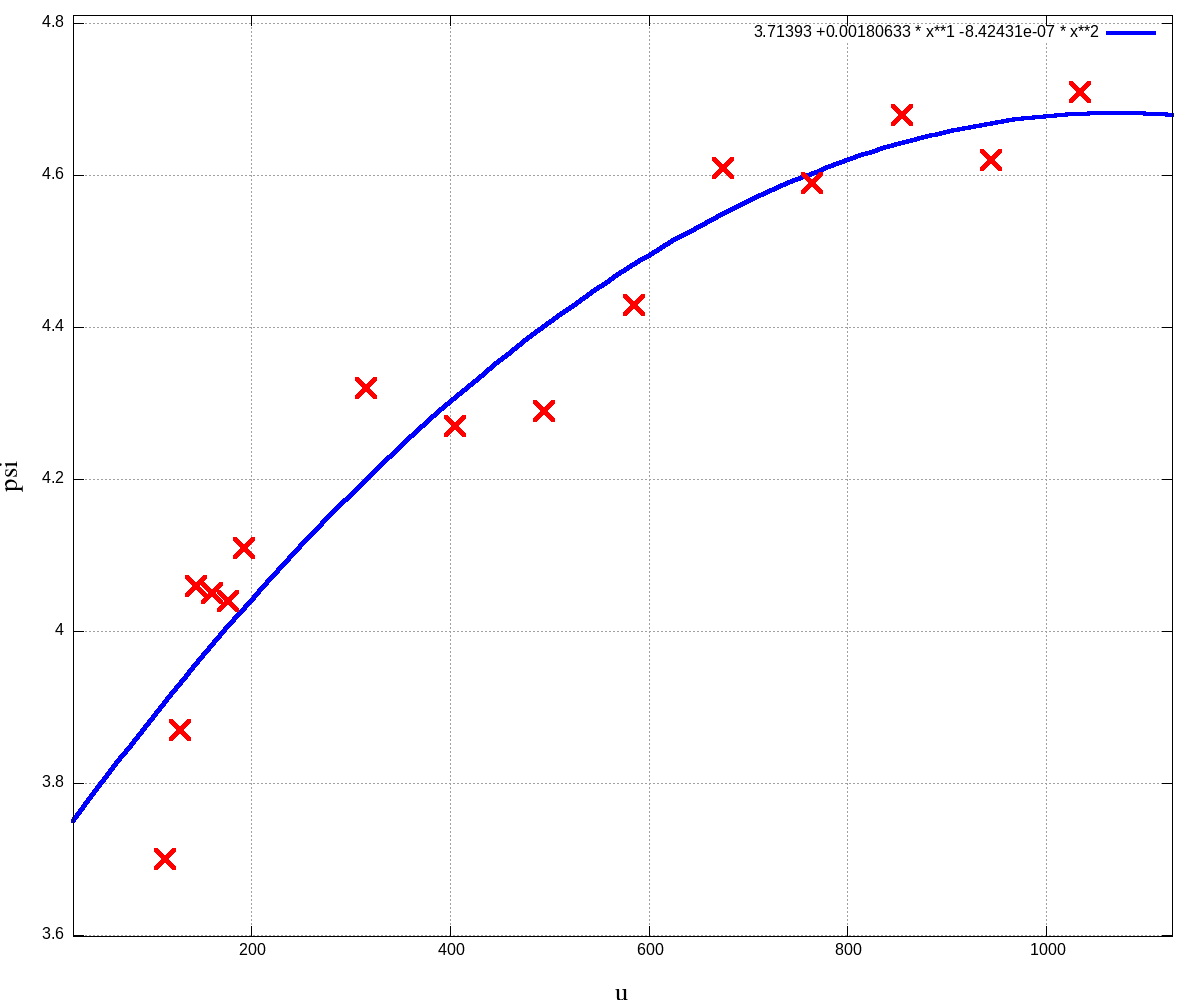
\includegraphics[width=0.8\textwidth]{3.png}
    \caption{график \( \psi(\nu) \)}
\end{figure}

Опроксимируем многочленом 2 степени:
\[ \psi = 3.7 + 0.002\nu -8.4\cdot 10^{-7}\nu^2\; rad \]

\subsection{Измерения в диапазоне \((0.5\nu_h - 15\nu_h)\)}
Исследуем зависимости \(\xi\) и \(\psi\) от \(\nu\):
\begin{table}[H]
    \centering
    \begin{tabular}{|c|c|c|c|c|}
    \hline
    \(\nu\), Hz & U, V  & I, A  & \(\psi\), rad & \(\xi = U/(\nu I)\) \\\hline
    1125  & 0.867 & 0.271 & 4.71 & 0.00284 \\\hline
    3330  & 0.468 & 0.148 & 5.02 & 0.0009  \\\hline
    5535  & 0.288 & 0.095 & 5.41 & 0.00055 \\\hline
    7740  & 0.197 & 0.068 & 5.80 & 0.0004  \\\hline
    9945  & 0.143 & 0.053 & 6.03 & 0.0003  \\\hline
    12150 & 0.106 & 0.041 & 6.13 & 0.00021 \\\hline
    14355 & 0.081 & 0.034 & 6.28 & 0.00017 \\\hline
    16560 & 0.062 & 0.028 & 6.70 & 0.00013 \\\hline
    18765 & 0.049 & 0.023 & 6.75 & 0.00011 \\\hline
    20970 & 0.039 & 0.019 & 7.07 & 9.8E-05 \\\hline
    23175 & 0.031 & 0.015 & 7.14 & 8.9E-05 \\\hline
    25380 & 0.026 & 0.012 & 4.55 & 8.5E-05 \\\hline
    27585 & 0.023 & 0.008 & 8.37 & 0.00010 \\\hline
    29790 & 0.022 & 0.006 & 8.50 & 0.00012 \\\hline
    31995 & 0.023 & 0.003 & 9.22 & 0.00024 \\\hline
    \end{tabular}
\end{table}

\begin{figure}[H]
    \centering
    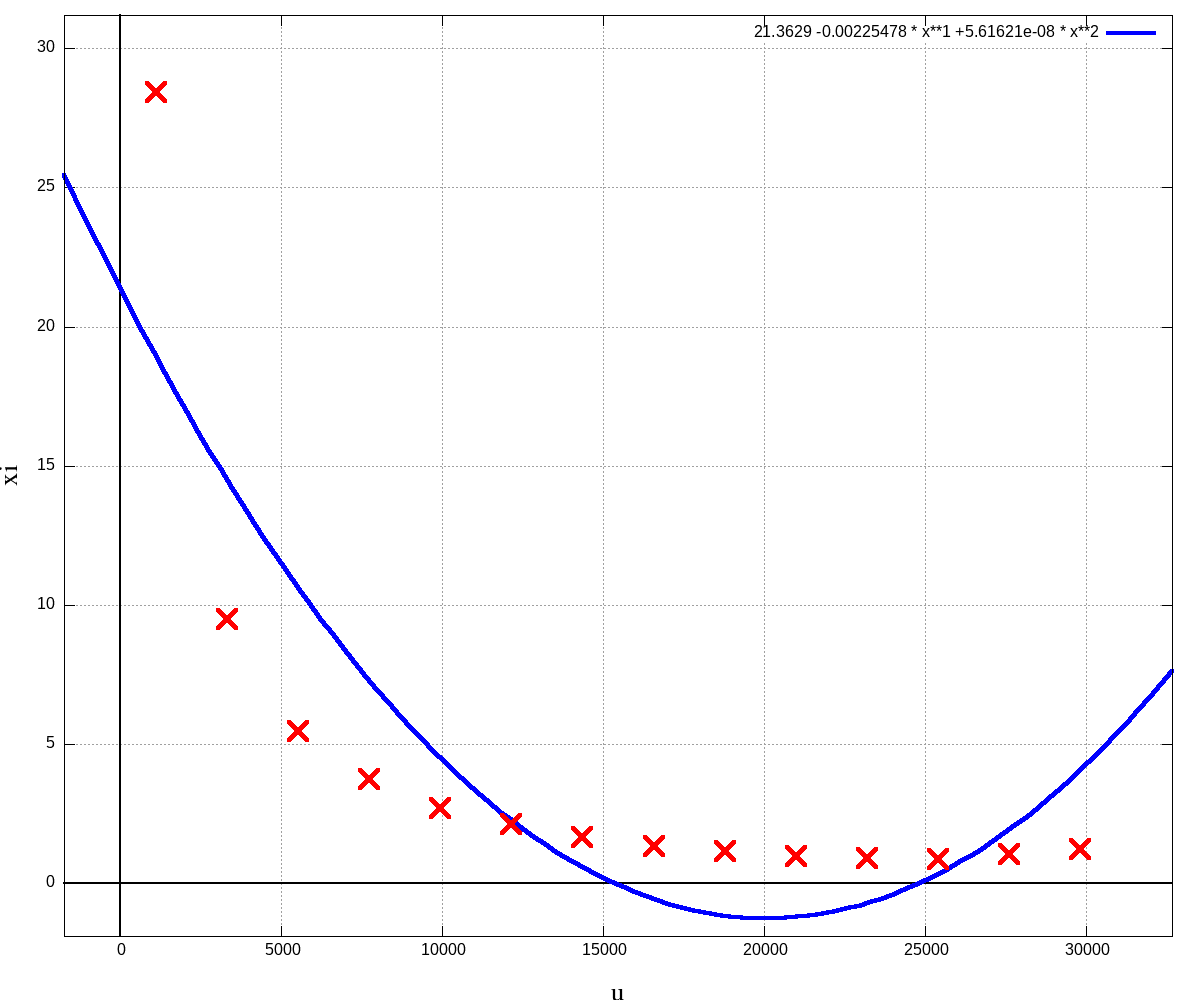
\includegraphics[width=0.8\textwidth]{4.png}
    \caption{график \( \xi(\nu) \)}
\end{figure}

Опроксимируем многочленом 2 степени:
\[ \xi = 21.4 - 0.0023\nu + 5.6\cdot 10^{-8}\nu^2 \]

\begin{figure}[H]
    \centering
    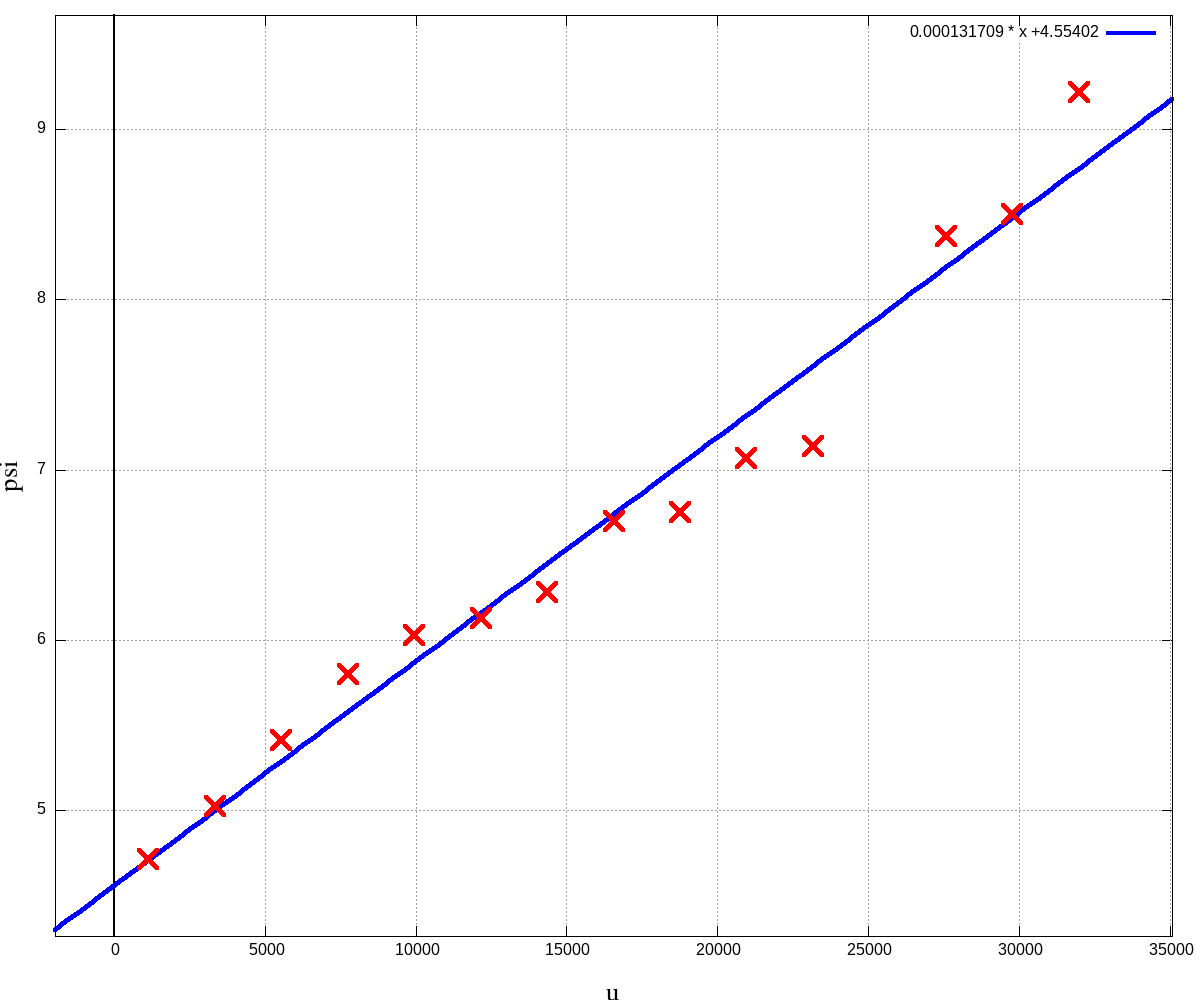
\includegraphics[width=0.8\textwidth]{5.png}
    \caption{график \( \psi(\nu) \)}
\end{figure}

Опроксимируем прямой вида \( \psi = a\nu + b \) :
\[ a = 1.3\cdot 10^{-4} \pm 6.3\cdot 10^{-6} \]
\[ b = 4.55 \pm 0.06 \]


\section{Выводы}


\end{document}